% Created by tikzDevice version 0.8.1 on 2015-08-28 10:31:17
% !TEX encoding = UTF-8 Unicode
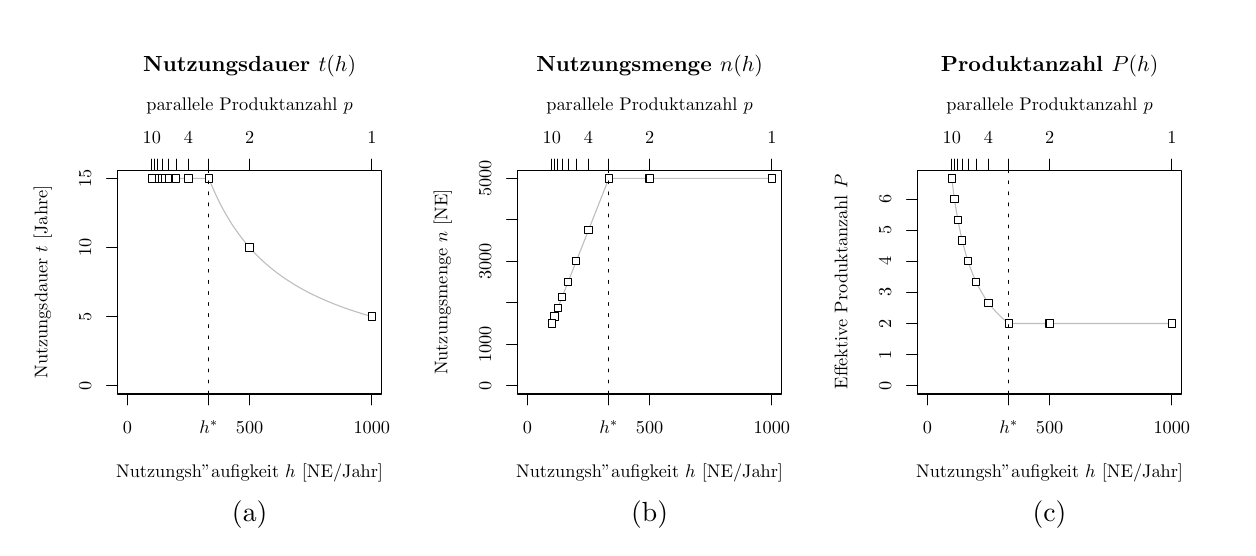
\begin{tikzpicture}[x=1pt,y=1pt]
\definecolor{fillColor}{RGB}{255,255,255}
\path[use as bounding box,fill=fillColor,fill opacity=0.00] (0,0) rectangle (433.62,180.67);
\begin{scope}
\path[clip] ( 32.47, 48.31) rectangle (127.91,129.19);
\definecolor{drawColor}{RGB}{190,190,190}

\path[draw=drawColor,line width= 0.4pt,line join=round,line cap=round] (124.37, 76.27) --
	(120.55, 77.40) --
	(117.04, 78.53) --
	(113.82, 79.66) --
	(110.84, 80.79) --
	(108.08, 81.92) --
	(105.51, 83.05) --
	(103.12, 84.17) --
	(100.90, 85.30) --
	( 98.81, 86.43) --
	( 96.85, 87.56) --
	( 95.02, 88.69) --
	( 93.29, 89.82) --
	( 91.66, 90.95) --
	( 90.11, 92.08) --
	( 88.66, 93.21) --
	( 87.27, 94.34) --
	( 85.96, 95.46) --
	( 84.72, 96.59) --
	( 83.53, 97.72) --
	( 82.40, 98.85) --
	( 81.33, 99.98) --
	( 80.30,101.11) --
	( 79.32,102.24) --
	( 78.38,103.37) --
	( 77.48,104.50) --
	( 76.62,105.63) --
	( 75.79,106.76) --
	( 75.00,107.88) --
	( 74.23,109.01) --
	( 73.50,110.14) --
	( 72.80,111.27) --
	( 72.12,112.40) --
	( 71.46,113.53) --
	( 70.83,114.66) --
	( 70.22,115.79) --
	( 69.63,116.92) --
	( 69.06,118.05) --
	( 68.51,119.17) --
	( 67.98,120.30) --
	( 67.46,121.43) --
	( 66.97,122.56) --
	( 66.48,123.69) --
	( 66.02,124.82) --
	( 65.56,125.95) --
	( 65.12,126.20) --
	( 64.69,126.20) --
	( 64.28,126.20) --
	( 63.88,126.20) --
	( 63.48,126.20) --
	( 63.10,126.20) --
	( 62.73,126.20) --
	( 62.37,126.20) --
	( 62.02,126.20) --
	( 61.68,126.20) --
	( 61.35,126.20) --
	( 61.02,126.20) --
	( 60.70,126.20) --
	( 60.40,126.20) --
	( 60.10,126.20) --
	( 59.80,126.20) --
	( 59.52,126.20) --
	( 59.24,126.20) --
	( 58.96,126.20) --
	( 58.70,126.20) --
	( 58.44,126.20) --
	( 58.18,126.20) --
	( 57.93,126.20) --
	( 57.69,126.20) --
	( 57.45,126.20) --
	( 57.22,126.20) --
	( 56.99,126.20) --
	( 56.77,126.20) --
	( 56.55,126.20) --
	( 56.34,126.20) --
	( 56.13,126.20) --
	( 55.92,126.20) --
	( 55.72,126.20) --
	( 55.52,126.20) --
	( 55.33,126.20) --
	( 55.14,126.20) --
	( 54.96,126.20) --
	( 54.77,126.20) --
	( 54.60,126.20) --
	( 54.42,126.20) --
	( 54.25,126.20) --
	( 54.08,126.20) --
	( 53.91,126.20) --
	( 53.75,126.20) --
	( 53.59,126.20) --
	( 53.43,126.20) --
	( 53.28,126.20) --
	( 53.13,126.20) --
	( 52.98,126.20) --
	( 52.83,126.20) --
	( 52.69,126.20) --
	( 52.55,126.20) --
	( 52.41,126.20) --
	( 52.27,126.20) --
	( 52.14,126.20) --
	( 52.01,126.20) --
	( 51.88,126.20) --
	( 51.75,126.20) --
	( 51.62,126.20) --
	( 51.50,126.20) --
	( 51.38,126.20) --
	( 51.26,126.20) --
	( 51.14,126.20) --
	( 51.02,126.20) --
	( 50.91,126.20) --
	( 50.80,126.20) --
	( 50.69,126.20) --
	( 50.58,126.20) --
	( 50.47,126.20) --
	( 50.36,126.20) --
	( 50.26,126.20) --
	( 50.15,126.20) --
	( 50.05,126.20) --
	( 49.95,126.20) --
	( 49.85,126.20) --
	( 49.76,126.20) --
	( 49.66,126.20) --
	( 49.56,126.20) --
	( 49.47,126.20) --
	( 49.38,126.20) --
	( 49.29,126.20) --
	( 49.20,126.20) --
	( 49.11,126.20) --
	( 49.02,126.20) --
	( 48.94,126.20) --
	( 48.85,126.20) --
	( 48.77,126.20) --
	( 48.69,126.20) --
	( 48.60,126.20) --
	( 48.52,126.20) --
	( 48.44,126.20) --
	( 48.36,126.20) --
	( 48.29,126.20) --
	( 48.21,126.20) --
	( 48.13,126.20) --
	( 48.06,126.20) --
	( 47.99,126.20) --
	( 47.91,126.20) --
	( 47.84,126.20) --
	( 47.77,126.20) --
	( 47.70,126.20) --
	( 47.63,126.20) --
	( 47.56,126.20) --
	( 47.49,126.20) --
	( 47.43,126.20) --
	( 47.36,126.20) --
	( 47.29,126.20) --
	( 47.23,126.20) --
	( 47.16,126.20) --
	( 47.10,126.20) --
	( 47.04,126.20) --
	( 46.98,126.20) --
	( 46.92,126.20) --
	( 46.85,126.20) --
	( 46.79,126.20) --
	( 46.74,126.20) --
	( 46.68,126.20) --
	( 46.62,126.20) --
	( 46.56,126.20) --
	( 46.51,126.20) --
	( 46.45,126.20) --
	( 46.39,126.20) --
	( 46.34,126.20) --
	( 46.28,126.20) --
	( 46.23,126.20) --
	( 46.18,126.20) --
	( 46.12,126.20) --
	( 46.07,126.20) --
	( 46.02,126.20) --
	( 45.97,126.20) --
	( 45.92,126.20) --
	( 45.87,126.20) --
	( 45.82,126.20) --
	( 45.77,126.20) --
	( 45.72,126.20) --
	( 45.67,126.20) --
	( 45.63,126.20) --
	( 45.58,126.20) --
	( 45.53,126.20) --
	( 45.49,126.20) --
	( 45.44,126.20) --
	( 45.40,126.20) --
	( 45.35,126.20) --
	( 45.31,126.20) --
	( 45.26,126.20) --
	( 45.22,126.20) --
	( 45.18,126.20) --
	( 45.13,126.20) --
	( 45.09,126.20) --
	( 45.05,126.20) --
	( 45.01,126.20) --
	( 44.96,126.20) --
	( 44.92,126.20) --
	( 44.88,126.20) --
	( 44.84,126.20);
\definecolor{drawColor}{RGB}{0,0,0}
\definecolor{fillColor}{RGB}{255,255,255}

\path[draw=drawColor,line width= 0.4pt,line join=round,line cap=round,fill=fillColor] (123.06, 74.96) rectangle (125.69, 77.59);

\path[draw=drawColor,line width= 0.4pt,line join=round,line cap=round,fill=fillColor] ( 78.87, 99.92) rectangle ( 81.51,102.55);

\path[draw=drawColor,line width= 0.4pt,line join=round,line cap=round,fill=fillColor] ( 64.15,124.88) rectangle ( 66.78,127.52);

\path[draw=drawColor,line width= 0.4pt,line join=round,line cap=round,fill=fillColor] ( 56.78,124.88) rectangle ( 59.41,127.52);

\path[draw=drawColor,line width= 0.4pt,line join=round,line cap=round,fill=fillColor] ( 52.36,124.88) rectangle ( 55.00,127.52);

\path[draw=drawColor,line width= 0.4pt,line join=round,line cap=round,fill=fillColor] ( 49.42,124.88) rectangle ( 52.05,127.52);

\path[draw=drawColor,line width= 0.4pt,line join=round,line cap=round,fill=fillColor] ( 47.31,124.88) rectangle ( 49.95,127.52);

\path[draw=drawColor,line width= 0.4pt,line join=round,line cap=round,fill=fillColor] ( 45.74,124.88) rectangle ( 48.37,127.52);

\path[draw=drawColor,line width= 0.4pt,line join=round,line cap=round,fill=fillColor] ( 44.51,124.88) rectangle ( 47.14,127.52);

\path[draw=drawColor,line width= 0.4pt,line join=round,line cap=round,fill=fillColor] ( 43.53,124.88) rectangle ( 46.16,127.52);
\end{scope}
\begin{scope}
\path[clip] (  0.00,  0.00) rectangle (144.54,180.67);
\definecolor{drawColor}{RGB}{0,0,0}

\node[text=drawColor,anchor=base,inner sep=0pt, outer sep=0pt, scale=  0.66] at ( 80.19, 18.22) {Nutzungsh"aufigkeit $h$ [NE/Jahr]};

\node[text=drawColor,rotate= 90.00,anchor=base,inner sep=0pt, outer sep=0pt, scale=  0.66] at (  7.13, 88.75) {Nutzungsdauer $t$ [Jahre]};
\end{scope}
\begin{scope}
\path[clip] ( 32.47, 48.31) rectangle (127.91,129.19);
\definecolor{drawColor}{RGB}{0,0,0}

\path[draw=drawColor,line width= 0.4pt,dash pattern=on 1pt off 3pt ,line join=round,line cap=round] ( 65.46, 48.31) -- ( 65.46,129.19);
\end{scope}
\begin{scope}
\path[clip] (  0.00,  0.00) rectangle (144.54,180.67);
\definecolor{drawColor}{RGB}{0,0,0}

\node[text=drawColor,anchor=base,inner sep=0pt, outer sep=0pt, scale=  0.79] at ( 80.19,164.83) {\bfseries Nutzungsdauer $t(h)$};
\end{scope}
\begin{scope}
\path[clip] (  0.00,  0.00) rectangle (433.62,180.67);
\definecolor{drawColor}{RGB}{0,0,0}

\path[draw=drawColor,line width= 0.4pt,line join=round,line cap=round] ( 36.01, 48.31) -- (124.37, 48.31);

\path[draw=drawColor,line width= 0.4pt,line join=round,line cap=round] ( 36.01, 48.31) -- ( 36.01, 44.35);

\path[draw=drawColor,line width= 0.4pt,line join=round,line cap=round] ( 65.46, 48.31) -- ( 65.46, 44.35);

\path[draw=drawColor,line width= 0.4pt,line join=round,line cap=round] ( 80.19, 48.31) -- ( 80.19, 44.35);

\path[draw=drawColor,line width= 0.4pt,line join=round,line cap=round] (124.37, 48.31) -- (124.37, 44.35);

\node[text=drawColor,anchor=base,inner sep=0pt, outer sep=0pt, scale=  0.66] at ( 36.01, 34.06) {0};

\node[text=drawColor,anchor=base,inner sep=0pt, outer sep=0pt, scale=  0.66] at ( 65.46, 34.06) {$h^*$};

\node[text=drawColor,anchor=base,inner sep=0pt, outer sep=0pt, scale=  0.66] at ( 80.19, 34.06) {500};

\node[text=drawColor,anchor=base,inner sep=0pt, outer sep=0pt, scale=  0.66] at (124.37, 34.06) {1000};

\path[draw=drawColor,line width= 0.4pt,line join=round,line cap=round] ( 32.47, 51.31) -- ( 32.47,126.20);

\path[draw=drawColor,line width= 0.4pt,line join=round,line cap=round] ( 32.47, 51.31) -- ( 28.51, 51.31);

\path[draw=drawColor,line width= 0.4pt,line join=round,line cap=round] ( 32.47, 76.27) -- ( 28.51, 76.27);

\path[draw=drawColor,line width= 0.4pt,line join=round,line cap=round] ( 32.47,101.24) -- ( 28.51,101.24);

\path[draw=drawColor,line width= 0.4pt,line join=round,line cap=round] ( 32.47,126.20) -- ( 28.51,126.20);

\node[text=drawColor,rotate= 90.00,anchor=base,inner sep=0pt, outer sep=0pt, scale=  0.66] at ( 22.97, 51.31) {0};

\node[text=drawColor,rotate= 90.00,anchor=base,inner sep=0pt, outer sep=0pt, scale=  0.66] at ( 22.97, 76.27) {5};

\node[text=drawColor,rotate= 90.00,anchor=base,inner sep=0pt, outer sep=0pt, scale=  0.66] at ( 22.97,101.24) {10};

\node[text=drawColor,rotate= 90.00,anchor=base,inner sep=0pt, outer sep=0pt, scale=  0.66] at ( 22.97,126.20) {15};

\path[draw=drawColor,line width= 0.4pt,line join=round,line cap=round] ( 44.84,129.19) -- (124.37,129.19);

\path[draw=drawColor,line width= 0.4pt,line join=round,line cap=round] ( 44.84,129.19) -- ( 44.84,133.15);

\path[draw=drawColor,line width= 0.4pt,line join=round,line cap=round] ( 45.83,129.19) -- ( 45.83,133.15);

\path[draw=drawColor,line width= 0.4pt,line join=round,line cap=round] ( 47.05,129.19) -- ( 47.05,133.15);

\path[draw=drawColor,line width= 0.4pt,line join=round,line cap=round] ( 48.63,129.19) -- ( 48.63,133.15);

\path[draw=drawColor,line width= 0.4pt,line join=round,line cap=round] ( 50.73,129.19) -- ( 50.73,133.15);

\path[draw=drawColor,line width= 0.4pt,line join=round,line cap=round] ( 53.68,129.19) -- ( 53.68,133.15);

\path[draw=drawColor,line width= 0.4pt,line join=round,line cap=round] ( 58.10,129.19) -- ( 58.10,133.15);

\path[draw=drawColor,line width= 0.4pt,line join=round,line cap=round] ( 65.46,129.19) -- ( 65.46,133.15);

\path[draw=drawColor,line width= 0.4pt,line join=round,line cap=round] ( 80.19,129.19) -- ( 80.19,133.15);

\path[draw=drawColor,line width= 0.4pt,line join=round,line cap=round] (124.37,129.19) -- (124.37,133.15);

\node[text=drawColor,anchor=base,inner sep=0pt, outer sep=0pt, scale=  0.66] at ( 44.84,138.70) {10};

\node[text=drawColor,anchor=base,inner sep=0pt, outer sep=0pt, scale=  0.66] at ( 58.10,138.70) {4};

\node[text=drawColor,anchor=base,inner sep=0pt, outer sep=0pt, scale=  0.66] at ( 80.19,138.70) {2};

\node[text=drawColor,anchor=base,inner sep=0pt, outer sep=0pt, scale=  0.66] at (124.37,138.70) {1};

\path[draw=drawColor,line width= 0.4pt,line join=round,line cap=round] ( 32.47, 48.31) --
	(127.91, 48.31) --
	(127.91,129.19) --
	( 32.47,129.19) --
	( 32.47, 48.31);

\node[text=drawColor,anchor=base,inner sep=0pt, outer sep=0pt, scale=  0.66] at ( 80.19,150.58) {parallele Produktanzahl $p$};

\node[text=drawColor,anchor=base,inner sep=0pt, outer sep=0pt, scale=  1.00] at ( 80.19,  2.38) {(a)};
\end{scope}
\begin{scope}
\path[clip] (177.01, 48.31) rectangle (272.45,129.19);
\definecolor{drawColor}{RGB}{190,190,190}

\path[draw=drawColor,line width= 0.4pt,line join=round,line cap=round] (268.91,126.20) --
	(265.09,126.20) --
	(261.58,126.20) --
	(258.36,126.20) --
	(255.38,126.20) --
	(252.62,126.20) --
	(250.05,126.20) --
	(247.66,126.20) --
	(245.44,126.20) --
	(243.35,126.20) --
	(241.39,126.20) --
	(239.56,126.20) --
	(237.83,126.20) --
	(236.20,126.20) --
	(234.65,126.20) --
	(233.20,126.20) --
	(231.81,126.20) --
	(230.50,126.20) --
	(229.26,126.20) --
	(228.07,126.20) --
	(226.94,126.20) --
	(225.87,126.20) --
	(224.84,126.20) --
	(223.86,126.20) --
	(222.92,126.20) --
	(222.02,126.20) --
	(221.16,126.20) --
	(220.33,126.20) --
	(219.54,126.20) --
	(218.77,126.20) --
	(218.04,126.20) --
	(217.34,126.20) --
	(216.66,126.20) --
	(216.00,126.20) --
	(215.37,126.20) --
	(214.76,126.20) --
	(214.17,126.20) --
	(213.60,126.20) --
	(213.05,126.20) --
	(212.52,126.20) --
	(212.00,126.20) --
	(211.51,126.20) --
	(211.02,126.20) --
	(210.56,126.20) --
	(210.10,126.20) --
	(209.66,125.33) --
	(209.23,124.24) --
	(208.82,123.19) --
	(208.42,122.16) --
	(208.02,121.17) --
	(207.64,120.20) --
	(207.27,119.26) --
	(206.91,118.34) --
	(206.56,117.45) --
	(206.22,116.58) --
	(205.89,115.73) --
	(205.56,114.91) --
	(205.24,114.10) --
	(204.94,113.32) --
	(204.64,112.55) --
	(204.34,111.81) --
	(204.06,111.08) --
	(203.78,110.37) --
	(203.50,109.68) --
	(203.24,109.00) --
	(202.98,108.34) --
	(202.72,107.69) --
	(202.47,107.06) --
	(202.23,106.44) --
	(201.99,105.83) --
	(201.76,105.24) --
	(201.53,104.66) --
	(201.31,104.09) --
	(201.09,103.54) --
	(200.88,103.00) --
	(200.67,102.46) --
	(200.46,101.94) --
	(200.26,101.43) --
	(200.06,100.93) --
	(199.87,100.44) --
	(199.68, 99.96) --
	(199.50, 99.49) --
	(199.31, 99.02) --
	(199.14, 98.57) --
	(198.96, 98.12) --
	(198.79, 97.69) --
	(198.62, 97.26) --
	(198.45, 96.84) --
	(198.29, 96.42) --
	(198.13, 96.02) --
	(197.97, 95.62) --
	(197.82, 95.23) --
	(197.67, 94.84) --
	(197.52, 94.46) --
	(197.37, 94.09) --
	(197.23, 93.73) --
	(197.09, 93.37) --
	(196.95, 93.02) --
	(196.81, 92.67) --
	(196.68, 92.33) --
	(196.55, 91.99) --
	(196.42, 91.66) --
	(196.29, 91.33) --
	(196.16, 91.01) --
	(196.04, 90.70) --
	(195.92, 90.39) --
	(195.80, 90.09) --
	(195.68, 89.78) --
	(195.56, 89.49) --
	(195.45, 89.20) --
	(195.34, 88.91) --
	(195.23, 88.63) --
	(195.12, 88.35) --
	(195.01, 88.08) --
	(194.90, 87.81) --
	(194.80, 87.54) --
	(194.69, 87.28) --
	(194.59, 87.02) --
	(194.49, 86.76) --
	(194.39, 86.51) --
	(194.30, 86.26) --
	(194.20, 86.02) --
	(194.10, 85.78) --
	(194.01, 85.54) --
	(193.92, 85.31) --
	(193.83, 85.08) --
	(193.74, 84.85) --
	(193.65, 84.62) --
	(193.56, 84.40) --
	(193.48, 84.18) --
	(193.39, 83.97) --
	(193.31, 83.75) --
	(193.23, 83.54) --
	(193.14, 83.34) --
	(193.06, 83.13) --
	(192.98, 82.93) --
	(192.90, 82.73) --
	(192.83, 82.53) --
	(192.75, 82.33) --
	(192.67, 82.14) --
	(192.60, 81.95) --
	(192.53, 81.76) --
	(192.45, 81.58) --
	(192.38, 81.40) --
	(192.31, 81.21) --
	(192.24, 81.04) --
	(192.17, 80.86) --
	(192.10, 80.68) --
	(192.03, 80.51) --
	(191.97, 80.34) --
	(191.90, 80.17) --
	(191.83, 80.00) --
	(191.77, 79.84) --
	(191.70, 79.68) --
	(191.64, 79.52) --
	(191.58, 79.36) --
	(191.52, 79.20) --
	(191.46, 79.04) --
	(191.39, 78.89) --
	(191.33, 78.74) --
	(191.28, 78.59) --
	(191.22, 78.44) --
	(191.16, 78.29) --
	(191.10, 78.14) --
	(191.05, 78.00) --
	(190.99, 77.86) --
	(190.93, 77.72) --
	(190.88, 77.58) --
	(190.82, 77.44) --
	(190.77, 77.30) --
	(190.72, 77.17) --
	(190.66, 77.03) --
	(190.61, 76.90) --
	(190.56, 76.77) --
	(190.51, 76.64) --
	(190.46, 76.51) --
	(190.41, 76.38) --
	(190.36, 76.26) --
	(190.31, 76.13) --
	(190.26, 76.01) --
	(190.21, 75.89) --
	(190.17, 75.77) --
	(190.12, 75.65) --
	(190.07, 75.53) --
	(190.03, 75.41) --
	(189.98, 75.29) --
	(189.94, 75.18) --
	(189.89, 75.06) --
	(189.85, 74.95) --
	(189.80, 74.84) --
	(189.76, 74.73) --
	(189.72, 74.62) --
	(189.67, 74.51) --
	(189.63, 74.40) --
	(189.59, 74.29) --
	(189.55, 74.19) --
	(189.50, 74.08) --
	(189.46, 73.98) --
	(189.42, 73.88) --
	(189.38, 73.78);
\definecolor{drawColor}{RGB}{0,0,0}
\definecolor{fillColor}{RGB}{255,255,255}

\path[draw=drawColor,line width= 0.4pt,line join=round,line cap=round,fill=fillColor] (267.60,124.88) rectangle (270.23,127.52);

\path[draw=drawColor,line width= 0.4pt,line join=round,line cap=round,fill=fillColor] (223.41,124.88) rectangle (226.05,127.52);

\path[draw=drawColor,line width= 0.4pt,line join=round,line cap=round,fill=fillColor] (208.69,124.88) rectangle (211.32,127.52);

\path[draw=drawColor,line width= 0.4pt,line join=round,line cap=round,fill=fillColor] (201.32,106.16) rectangle (203.95,108.79);

\path[draw=drawColor,line width= 0.4pt,line join=round,line cap=round,fill=fillColor] (196.90, 94.93) rectangle (199.54, 97.56);

\path[draw=drawColor,line width= 0.4pt,line join=round,line cap=round,fill=fillColor] (193.96, 87.44) rectangle (196.59, 90.07);

\path[draw=drawColor,line width= 0.4pt,line join=round,line cap=round,fill=fillColor] (191.85, 82.09) rectangle (194.49, 84.72);

\path[draw=drawColor,line width= 0.4pt,line join=round,line cap=round,fill=fillColor] (190.28, 78.08) rectangle (192.91, 80.71);

\path[draw=drawColor,line width= 0.4pt,line join=round,line cap=round,fill=fillColor] (189.05, 74.96) rectangle (191.68, 77.59);

\path[draw=drawColor,line width= 0.4pt,line join=round,line cap=round,fill=fillColor] (188.07, 72.46) rectangle (190.70, 75.09);
\end{scope}
\begin{scope}
\path[clip] (144.54,  0.00) rectangle (289.08,180.67);
\definecolor{drawColor}{RGB}{0,0,0}

\node[text=drawColor,anchor=base,inner sep=0pt, outer sep=0pt, scale=  0.66] at (224.73, 18.22) {Nutzungsh"aufigkeit $h$ [NE/Jahr]};

\node[text=drawColor,rotate= 90.00,anchor=base,inner sep=0pt, outer sep=0pt, scale=  0.66] at (151.67, 88.75) {Nutzungsmenge $n$ [NE]};
\end{scope}
\begin{scope}
\path[clip] (177.01, 48.31) rectangle (272.45,129.19);
\definecolor{drawColor}{RGB}{0,0,0}

\path[draw=drawColor,line width= 0.4pt,dash pattern=on 1pt off 3pt ,line join=round,line cap=round] (210.00, 48.31) -- (210.00,129.19);
\end{scope}
\begin{scope}
\path[clip] (144.54,  0.00) rectangle (289.08,180.67);
\definecolor{drawColor}{RGB}{0,0,0}

\node[text=drawColor,anchor=base,inner sep=0pt, outer sep=0pt, scale=  0.79] at (224.73,164.83) {\bfseries Nutzungsmenge $n(h)$};
\end{scope}
\begin{scope}
\path[clip] (  0.00,  0.00) rectangle (433.62,180.67);
\definecolor{drawColor}{RGB}{0,0,0}

\path[draw=drawColor,line width= 0.4pt,line join=round,line cap=round] (180.55, 48.31) -- (268.91, 48.31);

\path[draw=drawColor,line width= 0.4pt,line join=round,line cap=round] (180.55, 48.31) -- (180.55, 44.35);

\path[draw=drawColor,line width= 0.4pt,line join=round,line cap=round] (210.00, 48.31) -- (210.00, 44.35);

\path[draw=drawColor,line width= 0.4pt,line join=round,line cap=round] (224.73, 48.31) -- (224.73, 44.35);

\path[draw=drawColor,line width= 0.4pt,line join=round,line cap=round] (268.91, 48.31) -- (268.91, 44.35);

\node[text=drawColor,anchor=base,inner sep=0pt, outer sep=0pt, scale=  0.66] at (180.55, 34.06) {0};

\node[text=drawColor,anchor=base,inner sep=0pt, outer sep=0pt, scale=  0.66] at (210.00, 34.06) {$h^*$};

\node[text=drawColor,anchor=base,inner sep=0pt, outer sep=0pt, scale=  0.66] at (224.73, 34.06) {500};

\node[text=drawColor,anchor=base,inner sep=0pt, outer sep=0pt, scale=  0.66] at (268.91, 34.06) {1000};

\path[draw=drawColor,line width= 0.4pt,line join=round,line cap=round] (177.01, 51.31) -- (177.01,126.20);

\path[draw=drawColor,line width= 0.4pt,line join=round,line cap=round] (177.01, 51.31) -- (173.05, 51.31);

\path[draw=drawColor,line width= 0.4pt,line join=round,line cap=round] (177.01, 66.29) -- (173.05, 66.29);

\path[draw=drawColor,line width= 0.4pt,line join=round,line cap=round] (177.01, 81.26) -- (173.05, 81.26);

\path[draw=drawColor,line width= 0.4pt,line join=round,line cap=round] (177.01, 96.24) -- (173.05, 96.24);

\path[draw=drawColor,line width= 0.4pt,line join=round,line cap=round] (177.01,111.22) -- (173.05,111.22);

\path[draw=drawColor,line width= 0.4pt,line join=round,line cap=round] (177.01,126.20) -- (173.05,126.20);

\node[text=drawColor,rotate= 90.00,anchor=base,inner sep=0pt, outer sep=0pt, scale=  0.66] at (167.51, 51.31) {0};

\node[text=drawColor,rotate= 90.00,anchor=base,inner sep=0pt, outer sep=0pt, scale=  0.66] at (167.51, 66.29) {1000};

\node[text=drawColor,rotate= 90.00,anchor=base,inner sep=0pt, outer sep=0pt, scale=  0.66] at (167.51, 96.24) {3000};

\node[text=drawColor,rotate= 90.00,anchor=base,inner sep=0pt, outer sep=0pt, scale=  0.66] at (167.51,126.20) {5000};

\path[draw=drawColor,line width= 0.4pt,line join=round,line cap=round] (189.38,129.19) -- (268.91,129.19);

\path[draw=drawColor,line width= 0.4pt,line join=round,line cap=round] (189.38,129.19) -- (189.38,133.15);

\path[draw=drawColor,line width= 0.4pt,line join=round,line cap=round] (190.37,129.19) -- (190.37,133.15);

\path[draw=drawColor,line width= 0.4pt,line join=round,line cap=round] (191.59,129.19) -- (191.59,133.15);

\path[draw=drawColor,line width= 0.4pt,line join=round,line cap=round] (193.17,129.19) -- (193.17,133.15);

\path[draw=drawColor,line width= 0.4pt,line join=round,line cap=round] (195.27,129.19) -- (195.27,133.15);

\path[draw=drawColor,line width= 0.4pt,line join=round,line cap=round] (198.22,129.19) -- (198.22,133.15);

\path[draw=drawColor,line width= 0.4pt,line join=round,line cap=round] (202.64,129.19) -- (202.64,133.15);

\path[draw=drawColor,line width= 0.4pt,line join=round,line cap=round] (210.00,129.19) -- (210.00,133.15);

\path[draw=drawColor,line width= 0.4pt,line join=round,line cap=round] (224.73,129.19) -- (224.73,133.15);

\path[draw=drawColor,line width= 0.4pt,line join=round,line cap=round] (268.91,129.19) -- (268.91,133.15);

\node[text=drawColor,anchor=base,inner sep=0pt, outer sep=0pt, scale=  0.66] at (189.38,138.70) {10};

\node[text=drawColor,anchor=base,inner sep=0pt, outer sep=0pt, scale=  0.66] at (202.64,138.70) {4};

\node[text=drawColor,anchor=base,inner sep=0pt, outer sep=0pt, scale=  0.66] at (224.73,138.70) {2};

\node[text=drawColor,anchor=base,inner sep=0pt, outer sep=0pt, scale=  0.66] at (268.91,138.70) {1};

\path[draw=drawColor,line width= 0.4pt,line join=round,line cap=round] (177.01, 48.31) --
	(272.45, 48.31) --
	(272.45,129.19) --
	(177.01,129.19) --
	(177.01, 48.31);

\node[text=drawColor,anchor=base,inner sep=0pt, outer sep=0pt, scale=  0.66] at (224.73,150.58) {parallele Produktanzahl $p$};

\node[text=drawColor,anchor=base,inner sep=0pt, outer sep=0pt, scale=  1.00] at (224.73,  2.38) {(b)};
\end{scope}
\begin{scope}
\path[clip] (321.55, 48.31) rectangle (416.99,129.19);
\definecolor{drawColor}{RGB}{190,190,190}

\path[draw=drawColor,line width= 0.4pt,line join=round,line cap=round] (413.45, 73.78) --
	(409.63, 73.78) --
	(406.12, 73.78) --
	(402.90, 73.78) --
	(399.92, 73.78) --
	(397.16, 73.78) --
	(394.59, 73.78) --
	(392.20, 73.78) --
	(389.98, 73.78) --
	(387.89, 73.78) --
	(385.93, 73.78) --
	(384.10, 73.78) --
	(382.37, 73.78) --
	(380.74, 73.78) --
	(379.19, 73.78) --
	(377.74, 73.78) --
	(376.35, 73.78) --
	(375.04, 73.78) --
	(373.80, 73.78) --
	(372.61, 73.78) --
	(371.48, 73.78) --
	(370.41, 73.78) --
	(369.38, 73.78) --
	(368.40, 73.78) --
	(367.46, 73.78) --
	(366.56, 73.78) --
	(365.70, 73.78) --
	(364.87, 73.78) --
	(364.08, 73.78) --
	(363.31, 73.78) --
	(362.58, 73.78) --
	(361.88, 73.78) --
	(361.20, 73.78) --
	(360.54, 73.78) --
	(359.91, 73.78) --
	(359.30, 73.78) --
	(358.71, 73.78) --
	(358.14, 73.78) --
	(357.59, 73.78) --
	(357.06, 73.78) --
	(356.54, 73.78) --
	(356.05, 73.78) --
	(355.56, 73.78) --
	(355.10, 73.78) --
	(354.64, 73.78) --
	(354.20, 74.04) --
	(353.77, 74.38) --
	(353.36, 74.72) --
	(352.96, 75.05) --
	(352.56, 75.39) --
	(352.18, 75.73) --
	(351.81, 76.07) --
	(351.45, 76.41) --
	(351.10, 76.75) --
	(350.76, 77.09) --
	(350.43, 77.43) --
	(350.10, 77.76) --
	(349.78, 78.10) --
	(349.48, 78.44) --
	(349.18, 78.78) --
	(348.88, 79.12) --
	(348.60, 79.46) --
	(348.32, 79.80) --
	(348.04, 80.14) --
	(347.78, 80.47) --
	(347.52, 80.81) --
	(347.26, 81.15) --
	(347.01, 81.49) --
	(346.77, 81.83) --
	(346.53, 82.17) --
	(346.30, 82.51) --
	(346.07, 82.84) --
	(345.85, 83.18) --
	(345.63, 83.52) --
	(345.42, 83.86) --
	(345.21, 84.20) --
	(345.00, 84.54) --
	(344.80, 84.88) --
	(344.60, 85.22) --
	(344.41, 85.55) --
	(344.22, 85.89) --
	(344.04, 86.23) --
	(343.85, 86.57) --
	(343.68, 86.91) --
	(343.50, 87.25) --
	(343.33, 87.59) --
	(343.16, 87.93) --
	(342.99, 88.26) --
	(342.83, 88.60) --
	(342.67, 88.94) --
	(342.51, 89.28) --
	(342.36, 89.62) --
	(342.21, 89.96) --
	(342.06, 90.30) --
	(341.91, 90.64) --
	(341.77, 90.97) --
	(341.63, 91.31) --
	(341.49, 91.65) --
	(341.35, 91.99) --
	(341.22, 92.33) --
	(341.09, 92.67) --
	(340.96, 93.01) --
	(340.83, 93.34) --
	(340.70, 93.68) --
	(340.58, 94.02) --
	(340.46, 94.36) --
	(340.34, 94.70) --
	(340.22, 95.04) --
	(340.10, 95.38) --
	(339.99, 95.72) --
	(339.88, 96.05) --
	(339.77, 96.39) --
	(339.66, 96.73) --
	(339.55, 97.07) --
	(339.44, 97.41) --
	(339.34, 97.75) --
	(339.23, 98.09) --
	(339.13, 98.43) --
	(339.03, 98.76) --
	(338.93, 99.10) --
	(338.84, 99.44) --
	(338.74, 99.78) --
	(338.64,100.12) --
	(338.55,100.46) --
	(338.46,100.80) --
	(338.37,101.14) --
	(338.28,101.47) --
	(338.19,101.81) --
	(338.10,102.15) --
	(338.02,102.49) --
	(337.93,102.83) --
	(337.85,103.17) --
	(337.77,103.51) --
	(337.68,103.84) --
	(337.60,104.18) --
	(337.52,104.52) --
	(337.44,104.86) --
	(337.37,105.20) --
	(337.29,105.54) --
	(337.21,105.88) --
	(337.14,106.22) --
	(337.07,106.55) --
	(336.99,106.89) --
	(336.92,107.23) --
	(336.85,107.57) --
	(336.78,107.91) --
	(336.71,108.25) --
	(336.64,108.59) --
	(336.57,108.93) --
	(336.51,109.26) --
	(336.44,109.60) --
	(336.37,109.94) --
	(336.31,110.28) --
	(336.24,110.62) --
	(336.18,110.96) --
	(336.12,111.30) --
	(336.06,111.63) --
	(336.00,111.97) --
	(335.93,112.31) --
	(335.87,112.65) --
	(335.82,112.99) --
	(335.76,113.33) --
	(335.70,113.67) --
	(335.64,114.01) --
	(335.59,114.34) --
	(335.53,114.68) --
	(335.47,115.02) --
	(335.42,115.36) --
	(335.36,115.70) --
	(335.31,116.04) --
	(335.26,116.38) --
	(335.20,116.72) --
	(335.15,117.05) --
	(335.10,117.39) --
	(335.05,117.73) --
	(335.00,118.07) --
	(334.95,118.41) --
	(334.90,118.75) --
	(334.85,119.09) --
	(334.80,119.43) --
	(334.75,119.76) --
	(334.71,120.10) --
	(334.66,120.44) --
	(334.61,120.78) --
	(334.57,121.12) --
	(334.52,121.46) --
	(334.48,121.80) --
	(334.43,122.13) --
	(334.39,122.47) --
	(334.34,122.81) --
	(334.30,123.15) --
	(334.26,123.49) --
	(334.21,123.83) --
	(334.17,124.17) --
	(334.13,124.51) --
	(334.09,124.84) --
	(334.04,125.18) --
	(334.00,125.52) --
	(333.96,125.86) --
	(333.92,126.20);
\definecolor{drawColor}{RGB}{0,0,0}
\definecolor{fillColor}{RGB}{255,255,255}

\path[draw=drawColor,line width= 0.4pt,line join=round,line cap=round,fill=fillColor] (412.14, 72.46) rectangle (414.77, 75.09);

\path[draw=drawColor,line width= 0.4pt,line join=round,line cap=round,fill=fillColor] (367.95, 72.46) rectangle (370.59, 75.09);

\path[draw=drawColor,line width= 0.4pt,line join=round,line cap=round,fill=fillColor] (353.23, 72.46) rectangle (355.86, 75.09);

\path[draw=drawColor,line width= 0.4pt,line join=round,line cap=round,fill=fillColor] (345.86, 79.95) rectangle (348.49, 82.58);

\path[draw=drawColor,line width= 0.4pt,line join=round,line cap=round,fill=fillColor] (341.44, 87.44) rectangle (344.08, 90.07);

\path[draw=drawColor,line width= 0.4pt,line join=round,line cap=round,fill=fillColor] (338.50, 94.93) rectangle (341.13, 97.56);

\path[draw=drawColor,line width= 0.4pt,line join=round,line cap=round,fill=fillColor] (336.39,102.42) rectangle (339.03,105.05);

\path[draw=drawColor,line width= 0.4pt,line join=round,line cap=round,fill=fillColor] (334.82,109.90) rectangle (337.45,112.54);

\path[draw=drawColor,line width= 0.4pt,line join=round,line cap=round,fill=fillColor] (333.59,117.39) rectangle (336.22,120.03);

\path[draw=drawColor,line width= 0.4pt,line join=round,line cap=round,fill=fillColor] (332.61,124.88) rectangle (335.24,127.52);
\end{scope}
\begin{scope}
\path[clip] (289.08,  0.00) rectangle (433.62,180.67);
\definecolor{drawColor}{RGB}{0,0,0}

\node[text=drawColor,anchor=base,inner sep=0pt, outer sep=0pt, scale=  0.66] at (369.27, 18.22) {Nutzungsh"aufigkeit $h$ [NE/Jahr]};

\node[text=drawColor,rotate= 90.00,anchor=base,inner sep=0pt, outer sep=0pt, scale=  0.66] at (296.21, 88.75) {Effektive Produktanzahl $P$};
\end{scope}
\begin{scope}
\path[clip] (321.55, 48.31) rectangle (416.99,129.19);
\definecolor{drawColor}{RGB}{0,0,0}

\path[draw=drawColor,line width= 0.4pt,dash pattern=on 1pt off 3pt ,line join=round,line cap=round] (354.54, 48.31) -- (354.54,129.19);
\end{scope}
\begin{scope}
\path[clip] (289.08,  0.00) rectangle (433.62,180.67);
\definecolor{drawColor}{RGB}{0,0,0}

\node[text=drawColor,anchor=base,inner sep=0pt, outer sep=0pt, scale=  0.79] at (369.27,164.83) {\bfseries Produktanzahl $P(h)$};
\end{scope}
\begin{scope}
\path[clip] (  0.00,  0.00) rectangle (433.62,180.67);
\definecolor{drawColor}{RGB}{0,0,0}

\path[draw=drawColor,line width= 0.4pt,line join=round,line cap=round] (325.09, 48.31) -- (413.45, 48.31);

\path[draw=drawColor,line width= 0.4pt,line join=round,line cap=round] (325.09, 48.31) -- (325.09, 44.35);

\path[draw=drawColor,line width= 0.4pt,line join=round,line cap=round] (354.54, 48.31) -- (354.54, 44.35);

\path[draw=drawColor,line width= 0.4pt,line join=round,line cap=round] (369.27, 48.31) -- (369.27, 44.35);

\path[draw=drawColor,line width= 0.4pt,line join=round,line cap=round] (413.45, 48.31) -- (413.45, 44.35);

\node[text=drawColor,anchor=base,inner sep=0pt, outer sep=0pt, scale=  0.66] at (325.09, 34.06) {0};

\node[text=drawColor,anchor=base,inner sep=0pt, outer sep=0pt, scale=  0.66] at (354.54, 34.06) {$h^*$};

\node[text=drawColor,anchor=base,inner sep=0pt, outer sep=0pt, scale=  0.66] at (369.27, 34.06) {500};

\node[text=drawColor,anchor=base,inner sep=0pt, outer sep=0pt, scale=  0.66] at (413.45, 34.06) {1000};

\path[draw=drawColor,line width= 0.4pt,line join=round,line cap=round] (321.55, 51.31) -- (321.55,118.71);

\path[draw=drawColor,line width= 0.4pt,line join=round,line cap=round] (321.55, 51.31) -- (317.59, 51.31);

\path[draw=drawColor,line width= 0.4pt,line join=round,line cap=round] (321.55, 62.54) -- (317.59, 62.54);

\path[draw=drawColor,line width= 0.4pt,line join=round,line cap=round] (321.55, 73.78) -- (317.59, 73.78);

\path[draw=drawColor,line width= 0.4pt,line join=round,line cap=round] (321.55, 85.01) -- (317.59, 85.01);

\path[draw=drawColor,line width= 0.4pt,line join=round,line cap=round] (321.55, 96.24) -- (317.59, 96.24);

\path[draw=drawColor,line width= 0.4pt,line join=round,line cap=round] (321.55,107.48) -- (317.59,107.48);

\path[draw=drawColor,line width= 0.4pt,line join=round,line cap=round] (321.55,118.71) -- (317.59,118.71);

\node[text=drawColor,rotate= 90.00,anchor=base,inner sep=0pt, outer sep=0pt, scale=  0.66] at (312.05, 51.31) {0};

\node[text=drawColor,rotate= 90.00,anchor=base,inner sep=0pt, outer sep=0pt, scale=  0.66] at (312.05, 62.54) {1};

\node[text=drawColor,rotate= 90.00,anchor=base,inner sep=0pt, outer sep=0pt, scale=  0.66] at (312.05, 73.78) {2};

\node[text=drawColor,rotate= 90.00,anchor=base,inner sep=0pt, outer sep=0pt, scale=  0.66] at (312.05, 85.01) {3};

\node[text=drawColor,rotate= 90.00,anchor=base,inner sep=0pt, outer sep=0pt, scale=  0.66] at (312.05, 96.24) {4};

\node[text=drawColor,rotate= 90.00,anchor=base,inner sep=0pt, outer sep=0pt, scale=  0.66] at (312.05,107.48) {5};

\node[text=drawColor,rotate= 90.00,anchor=base,inner sep=0pt, outer sep=0pt, scale=  0.66] at (312.05,118.71) {6};

\path[draw=drawColor,line width= 0.4pt,line join=round,line cap=round] (333.92,129.19) -- (413.45,129.19);

\path[draw=drawColor,line width= 0.4pt,line join=round,line cap=round] (333.92,129.19) -- (333.92,133.15);

\path[draw=drawColor,line width= 0.4pt,line join=round,line cap=round] (334.91,129.19) -- (334.91,133.15);

\path[draw=drawColor,line width= 0.4pt,line join=round,line cap=round] (336.13,129.19) -- (336.13,133.15);

\path[draw=drawColor,line width= 0.4pt,line join=round,line cap=round] (337.71,129.19) -- (337.71,133.15);

\path[draw=drawColor,line width= 0.4pt,line join=round,line cap=round] (339.81,129.19) -- (339.81,133.15);

\path[draw=drawColor,line width= 0.4pt,line join=round,line cap=round] (342.76,129.19) -- (342.76,133.15);

\path[draw=drawColor,line width= 0.4pt,line join=round,line cap=round] (347.18,129.19) -- (347.18,133.15);

\path[draw=drawColor,line width= 0.4pt,line join=round,line cap=round] (354.54,129.19) -- (354.54,133.15);

\path[draw=drawColor,line width= 0.4pt,line join=round,line cap=round] (369.27,129.19) -- (369.27,133.15);

\path[draw=drawColor,line width= 0.4pt,line join=round,line cap=round] (413.45,129.19) -- (413.45,133.15);

\node[text=drawColor,anchor=base,inner sep=0pt, outer sep=0pt, scale=  0.66] at (333.92,138.70) {10};

\node[text=drawColor,anchor=base,inner sep=0pt, outer sep=0pt, scale=  0.66] at (347.18,138.70) {4};

\node[text=drawColor,anchor=base,inner sep=0pt, outer sep=0pt, scale=  0.66] at (369.27,138.70) {2};

\node[text=drawColor,anchor=base,inner sep=0pt, outer sep=0pt, scale=  0.66] at (413.45,138.70) {1};

\path[draw=drawColor,line width= 0.4pt,line join=round,line cap=round] (321.55, 48.31) --
	(416.99, 48.31) --
	(416.99,129.19) --
	(321.55,129.19) --
	(321.55, 48.31);

\node[text=drawColor,anchor=base,inner sep=0pt, outer sep=0pt, scale=  0.66] at (369.27,150.58) {parallele Produktanzahl $p$};

\node[text=drawColor,anchor=base,inner sep=0pt, outer sep=0pt, scale=  1.00] at (369.27,  2.38) {(c)};
\end{scope}
\end{tikzpicture}
